\documentclass[aspectratio=169, professionalfonts]{beamer}
\usetheme[progressbar=frametitle]{metropolis}

\usepackage{appendixnumberbeamer}
\usepackage{booktabs}
\usepackage{caption}
\usepackage[scale=2]{ccicons}
\usepackage{outlines}
\usepackage{polyglossia}
\usepackage{subcaption}
\usepackage{unicode-math}
\usepackage{xspace}

\setmainlanguage[babelshorthands=true]{russian}
\setotherlanguage{english}
\defaultfontfeatures{Renderer=Basic, Ligatures=TeX}
\newfontfamily\cyrillicfonttt{CMU Typewriter Text}
\newfontfamily\cyrillicfont{CMU Sans Serif}
\setmainfont{CMU Sans Serif}
\setsansfont{CMU Sans Serif}
\setmonofont{CMU Typewriter Text}
\setmathfont{XITS Math}

\title{Лекция 2. Классические задачи машинного обучения}
\date{Введение в нейронные сети | 10.10.2023}

\begin{document}

\maketitle

\begin{frame}{Классификация методов}
    \centering
    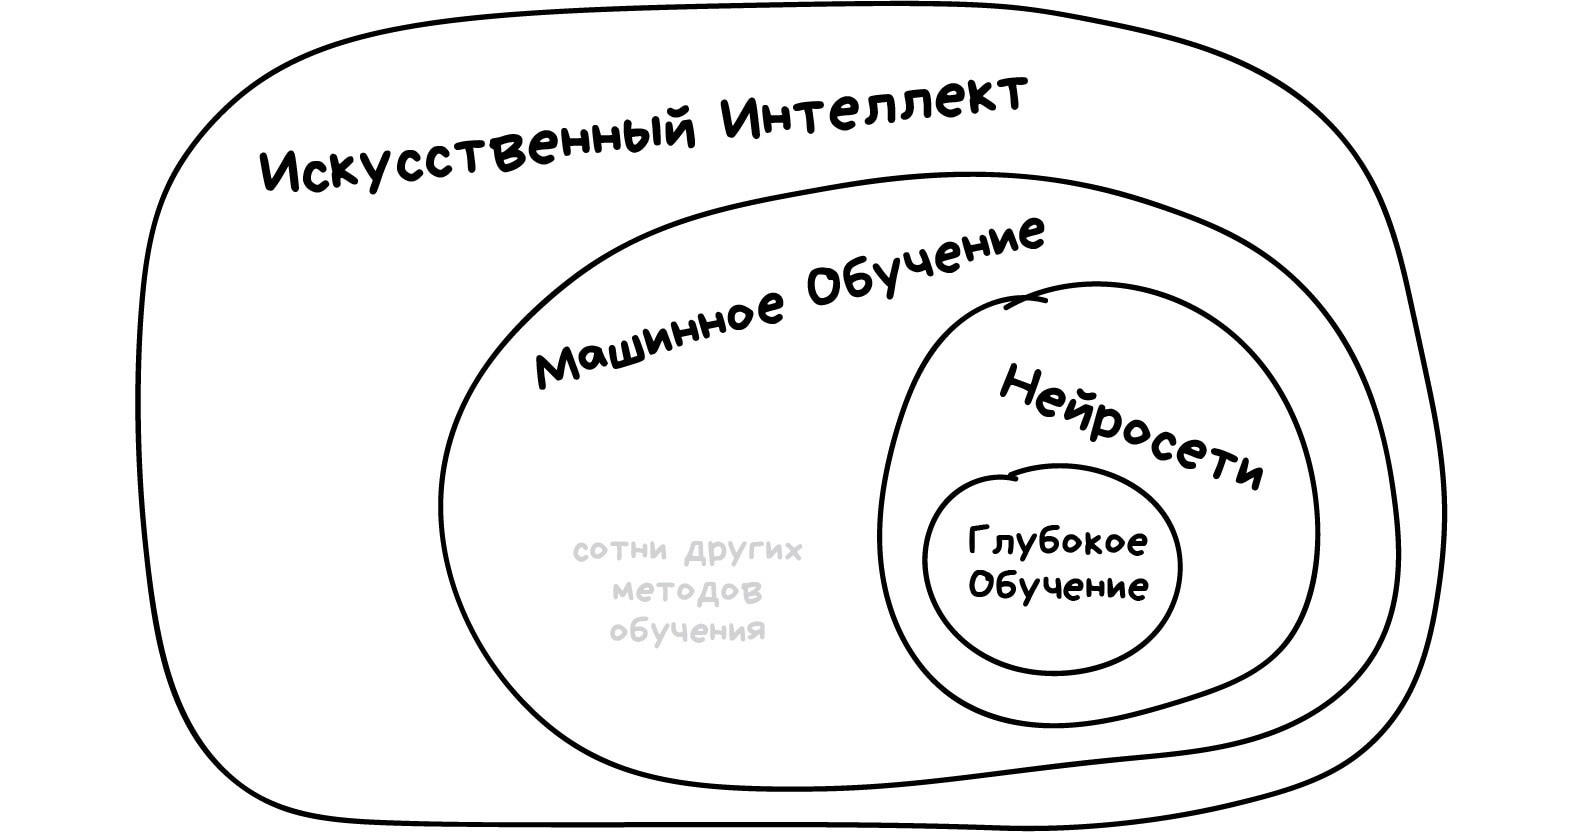
\includegraphics[width=.9\linewidth]{figures/fig1-terms.jpg}
\end{frame}

\begin{frame}{Особенности ML задач}
    \begin{outline}
        \1 Их решение (или часть решения) можно записать как функцию, которая отображает
        \textbf{объекты} (примеры, samples) в \textbf{предсказания} (targets)
            \2 \( f("Hello \ world!") \to \) "Привет, мир!"
            \2 \( f(netflix \ history) \to \) [Кибердеревня (сериал 2023)]
            \2 \( f(t = 37^\circ C) \to \) вы больны с вероятностью 0.5
        \1 Можно собрать примеры правильных и неправильных ответов
        \1 Подходит не идеальное, а достаточно хорошее решение
            (люди тоже нередко ошибаются)
    \end{outline}
\end{frame}

\begin{frame}{Computer Science vs. Data Driven (ML)}
    \begin{columns}[T]
        \begin{column}{.49\linewidth}
            \centering
            Computer Science \& Software Engineering
            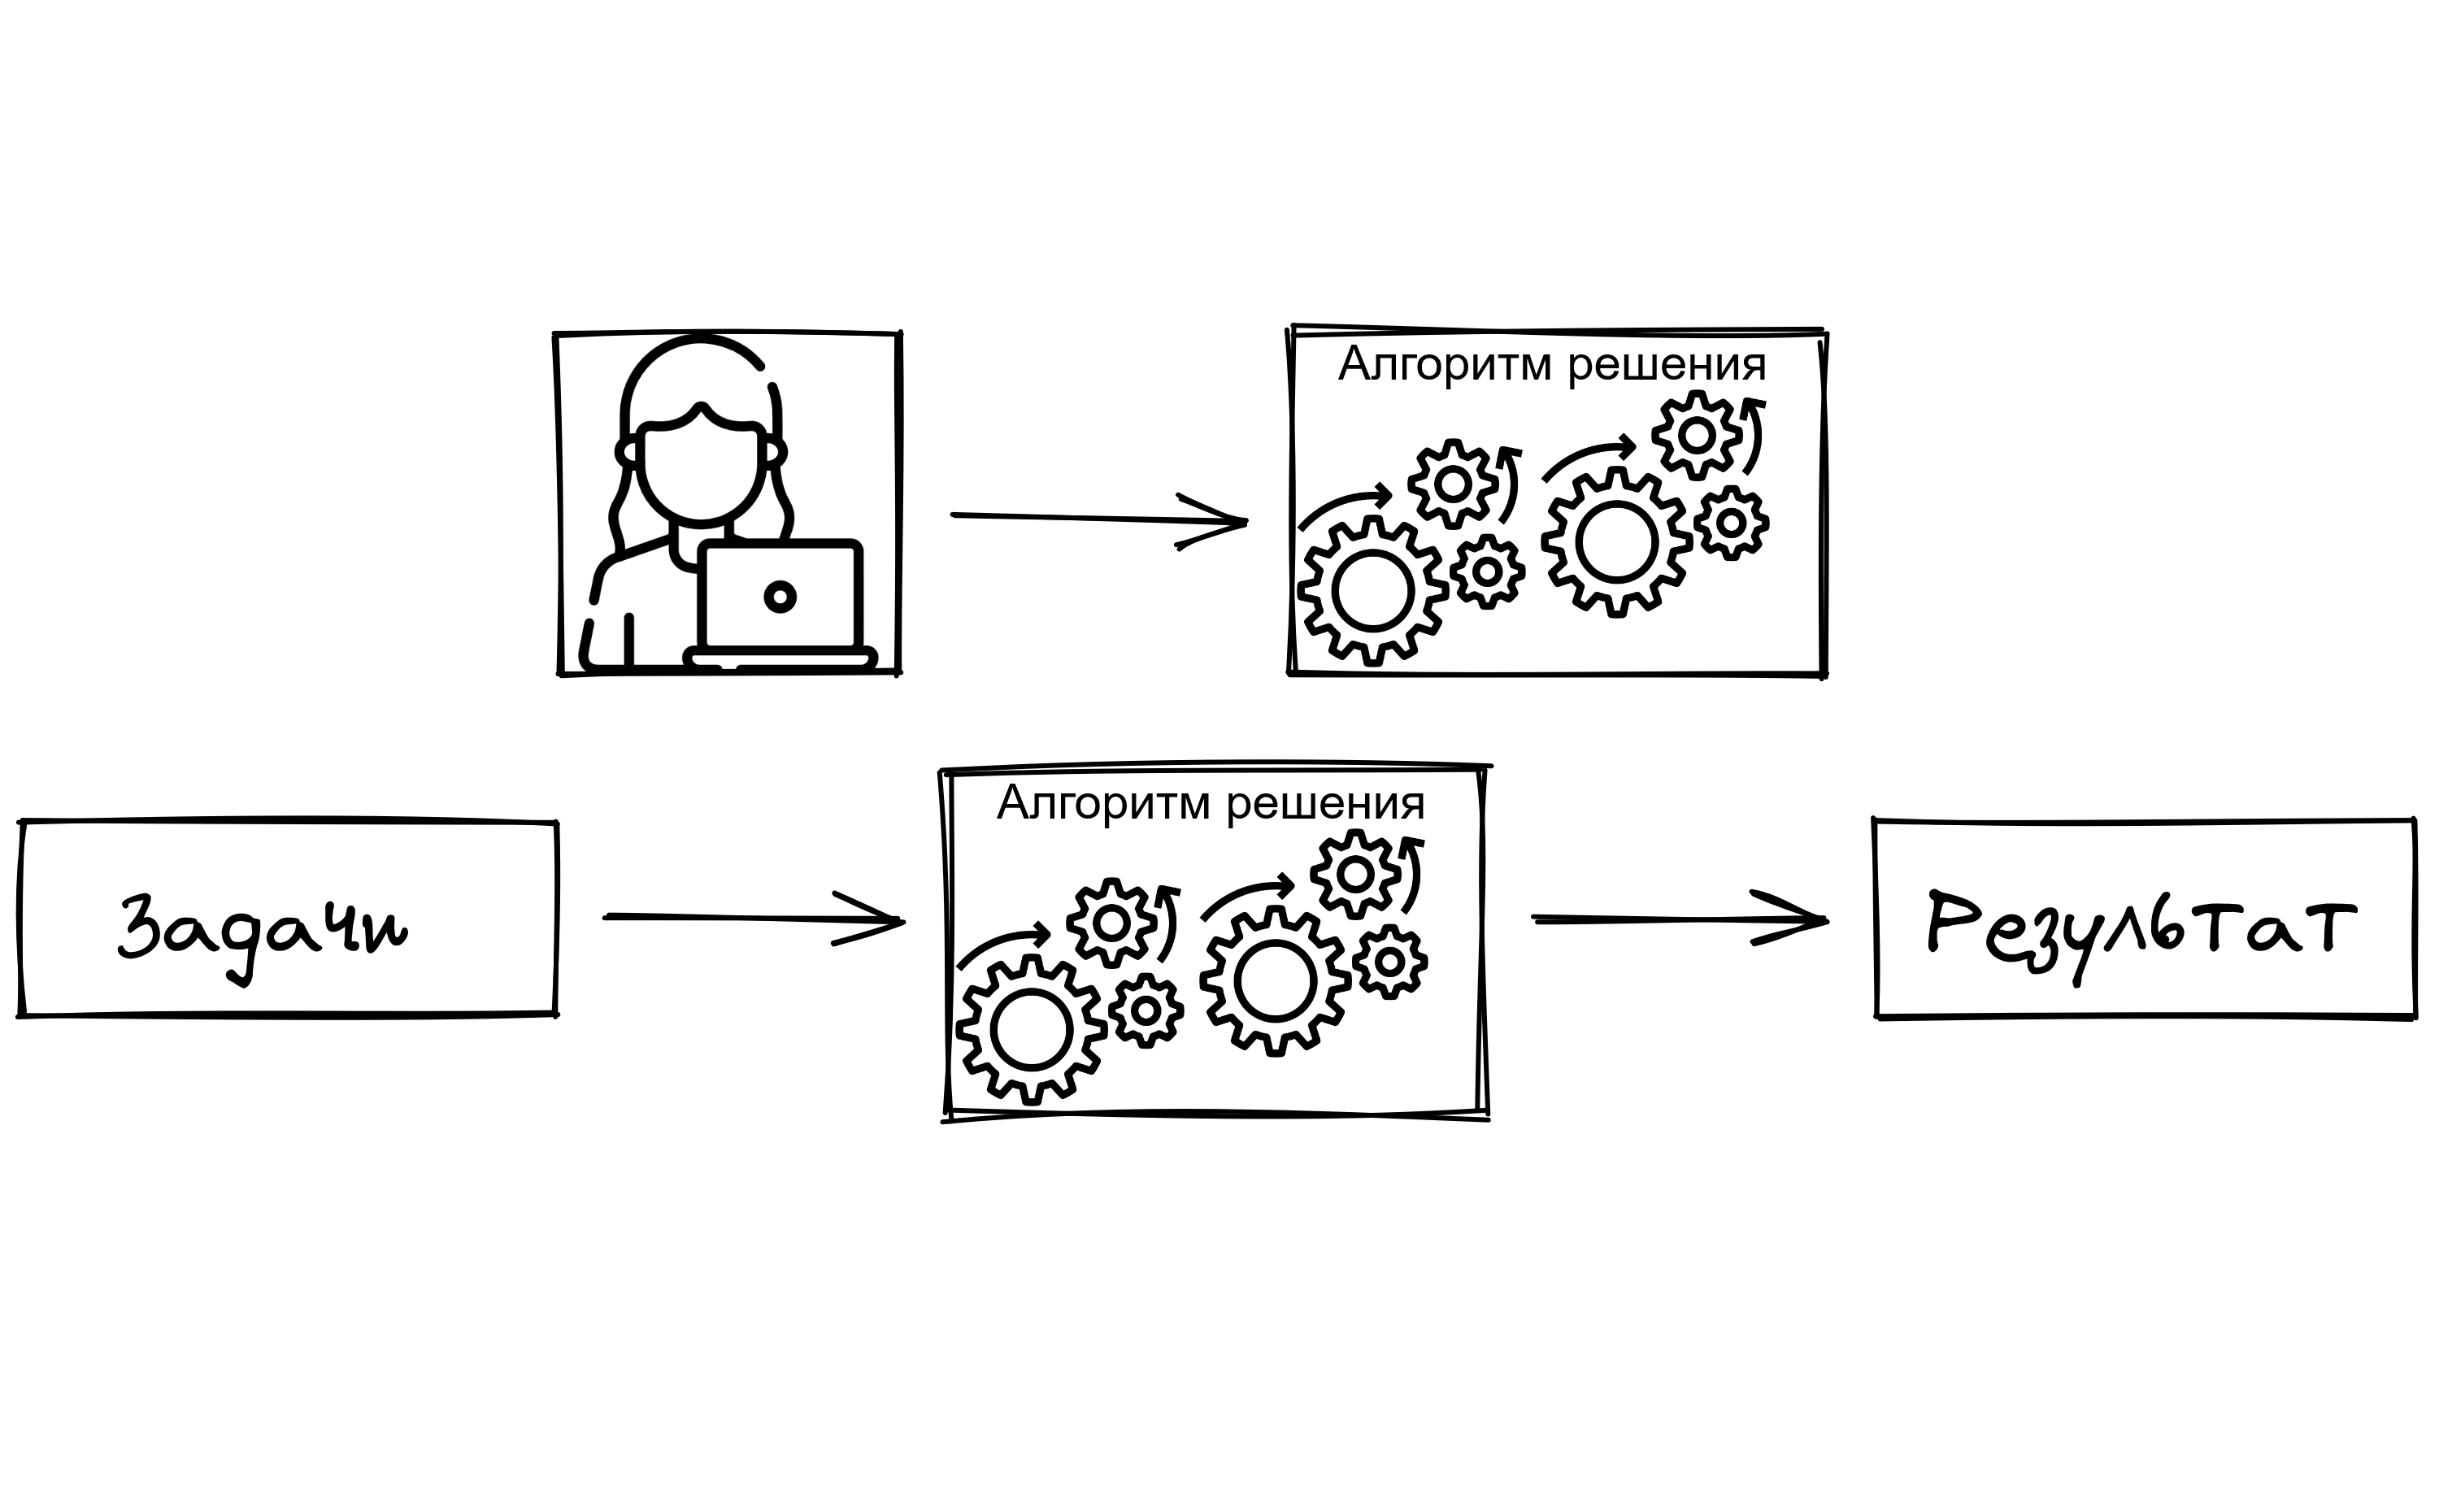
\includegraphics[width=\linewidth]{figures/fig2-swe.jpg}
        \end{column}
        \begin{column}{.49\linewidth}
            \centering
            Machine Learning
            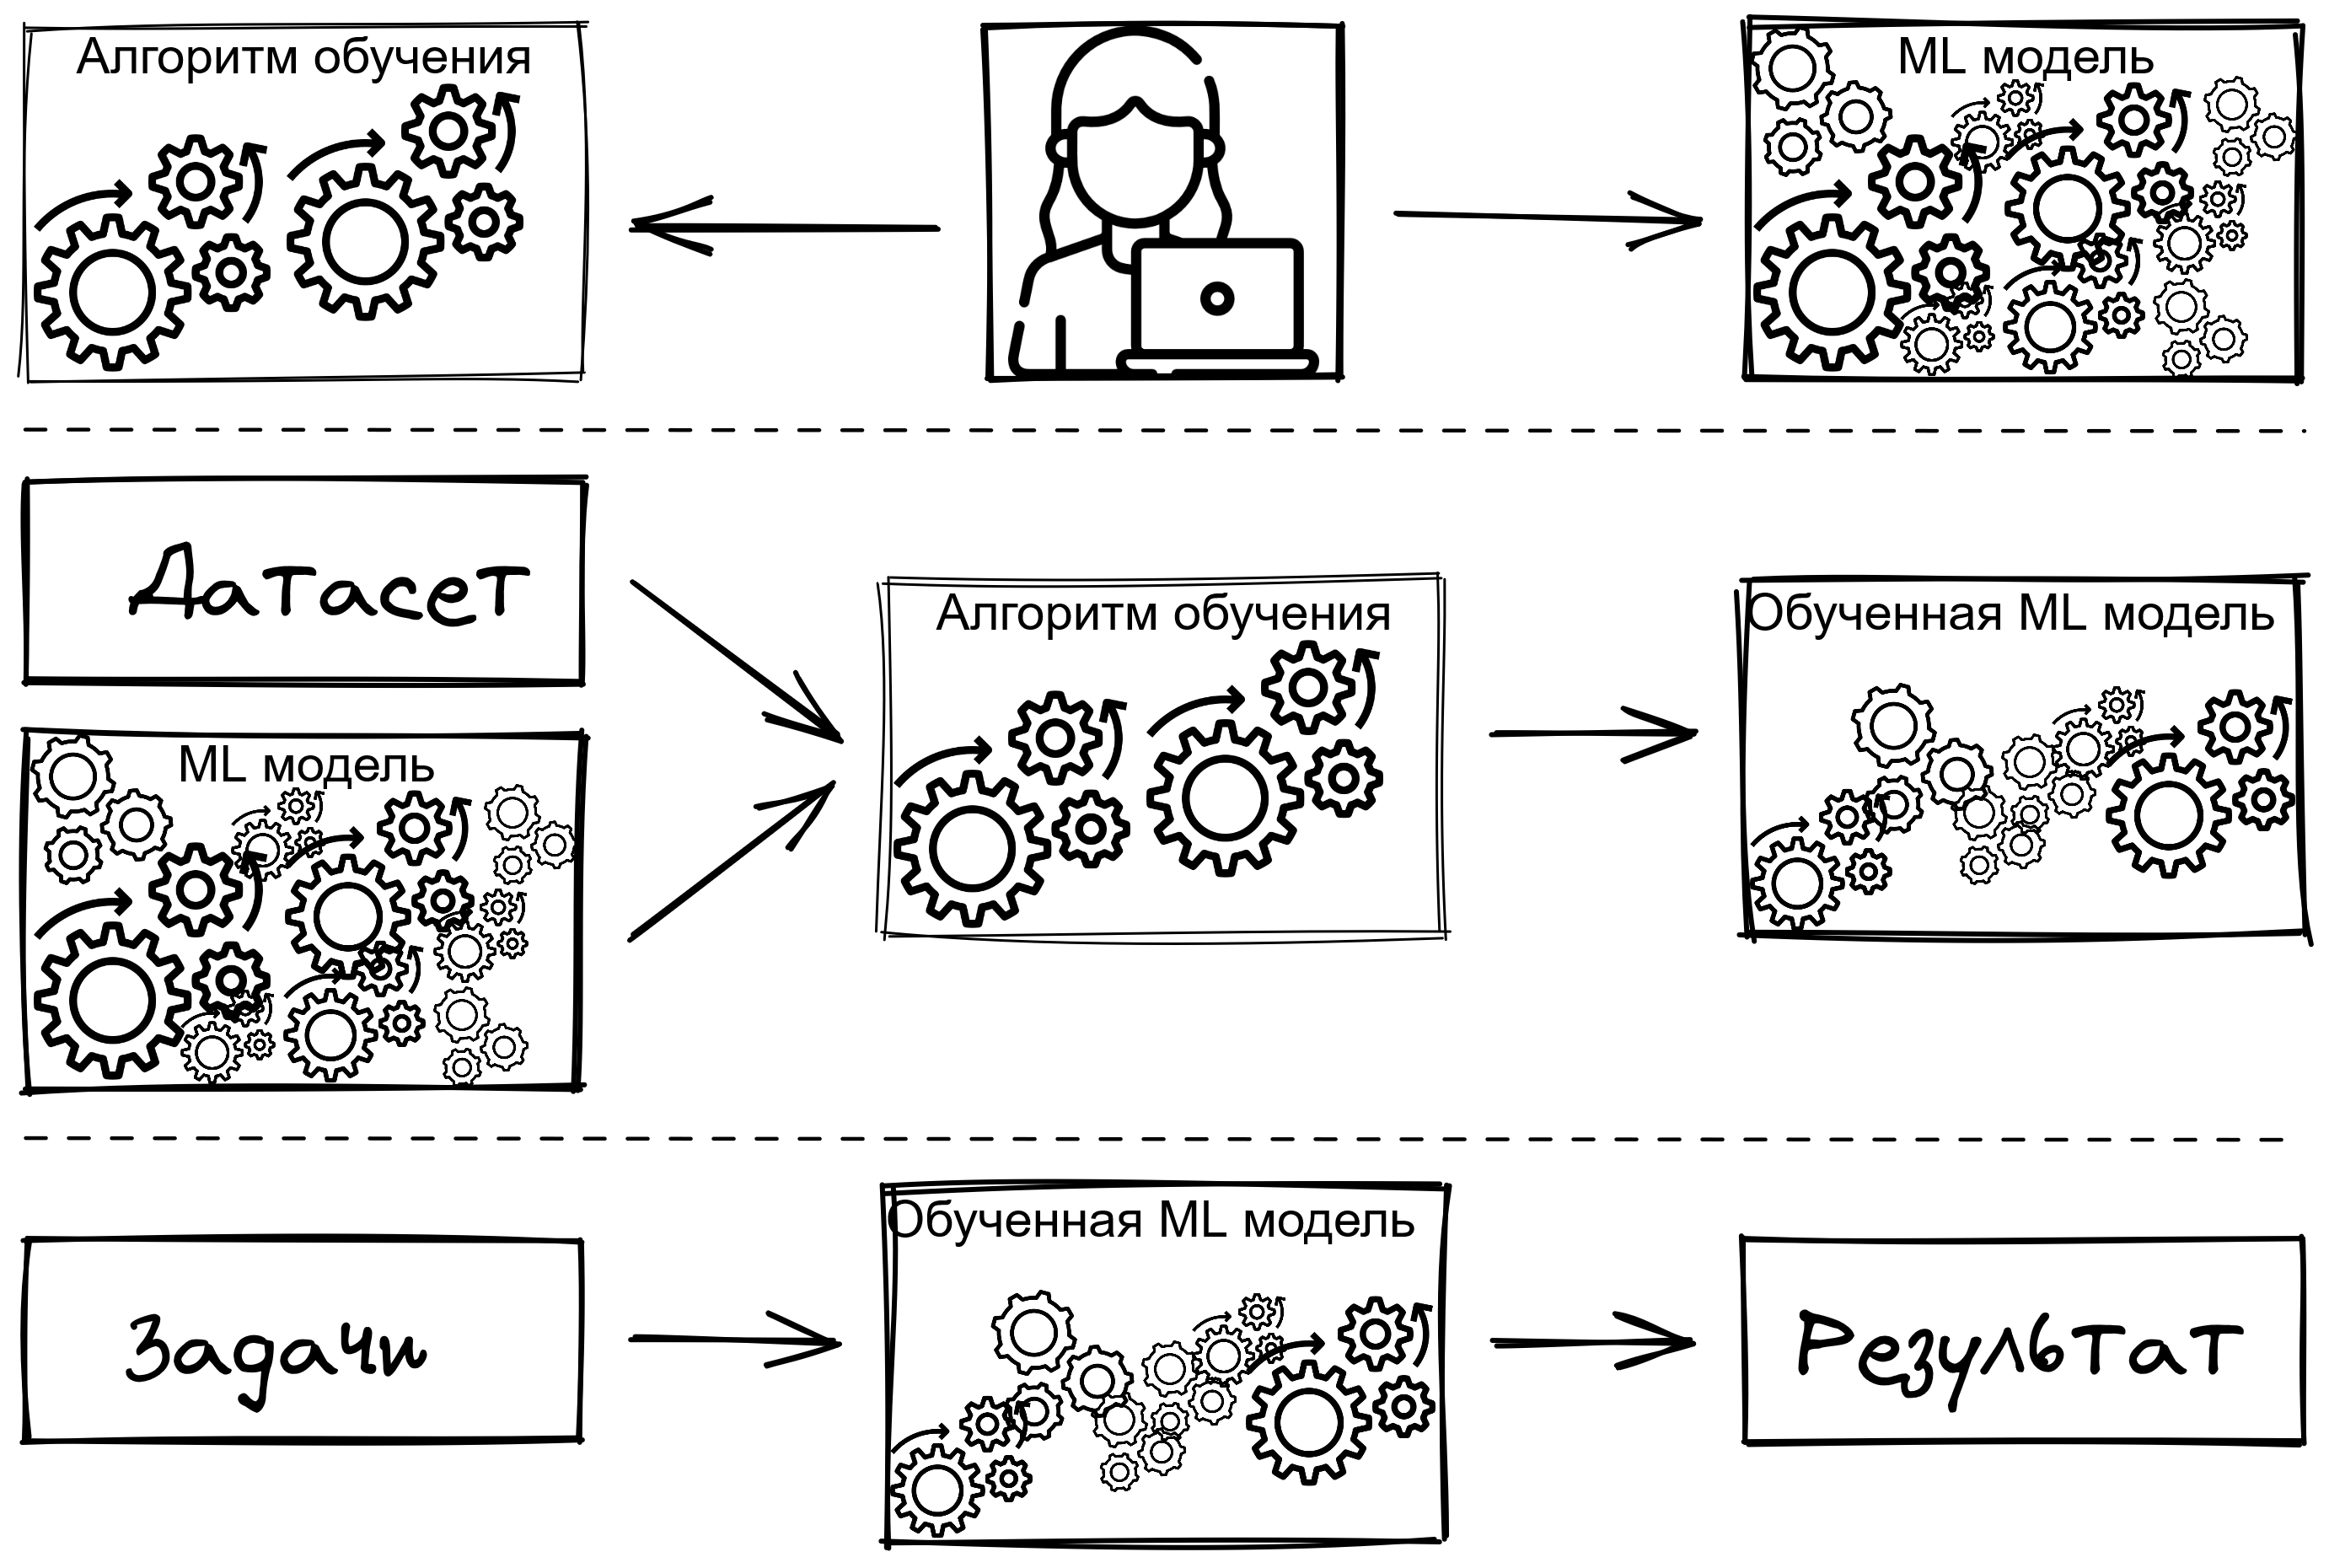
\includegraphics[width=\linewidth]{figures/fig3-mle.jpg}
        \end{column}
    \end{columns}
\end{frame}

\begin{frame}{Задачи машинного обучения}
    \centering
    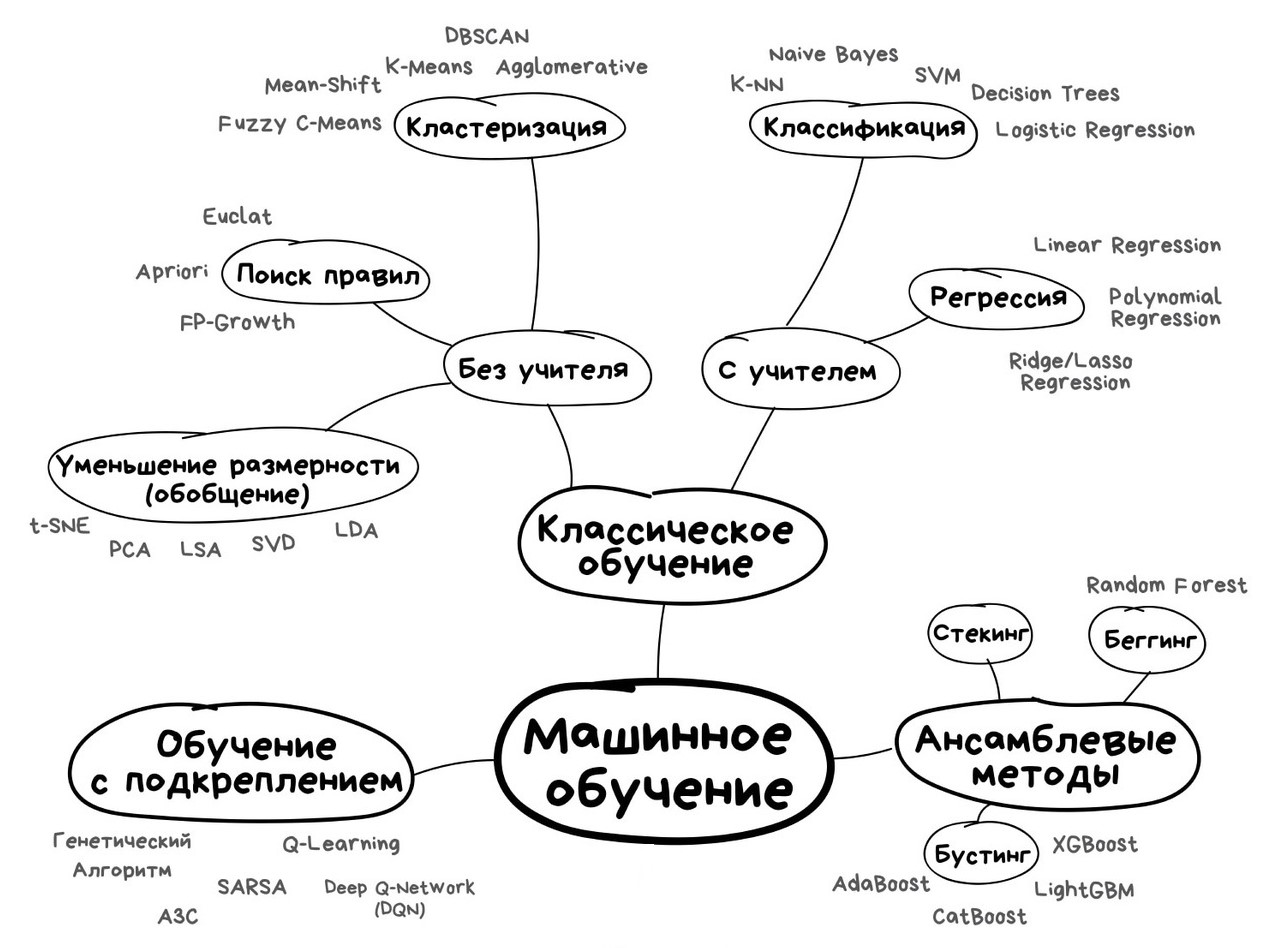
\includegraphics[width=.65\linewidth]{figures/fig4-tasks.jpg}
\end{frame}

\begin{frame}{Задачи машинного обучения}
    \centering
    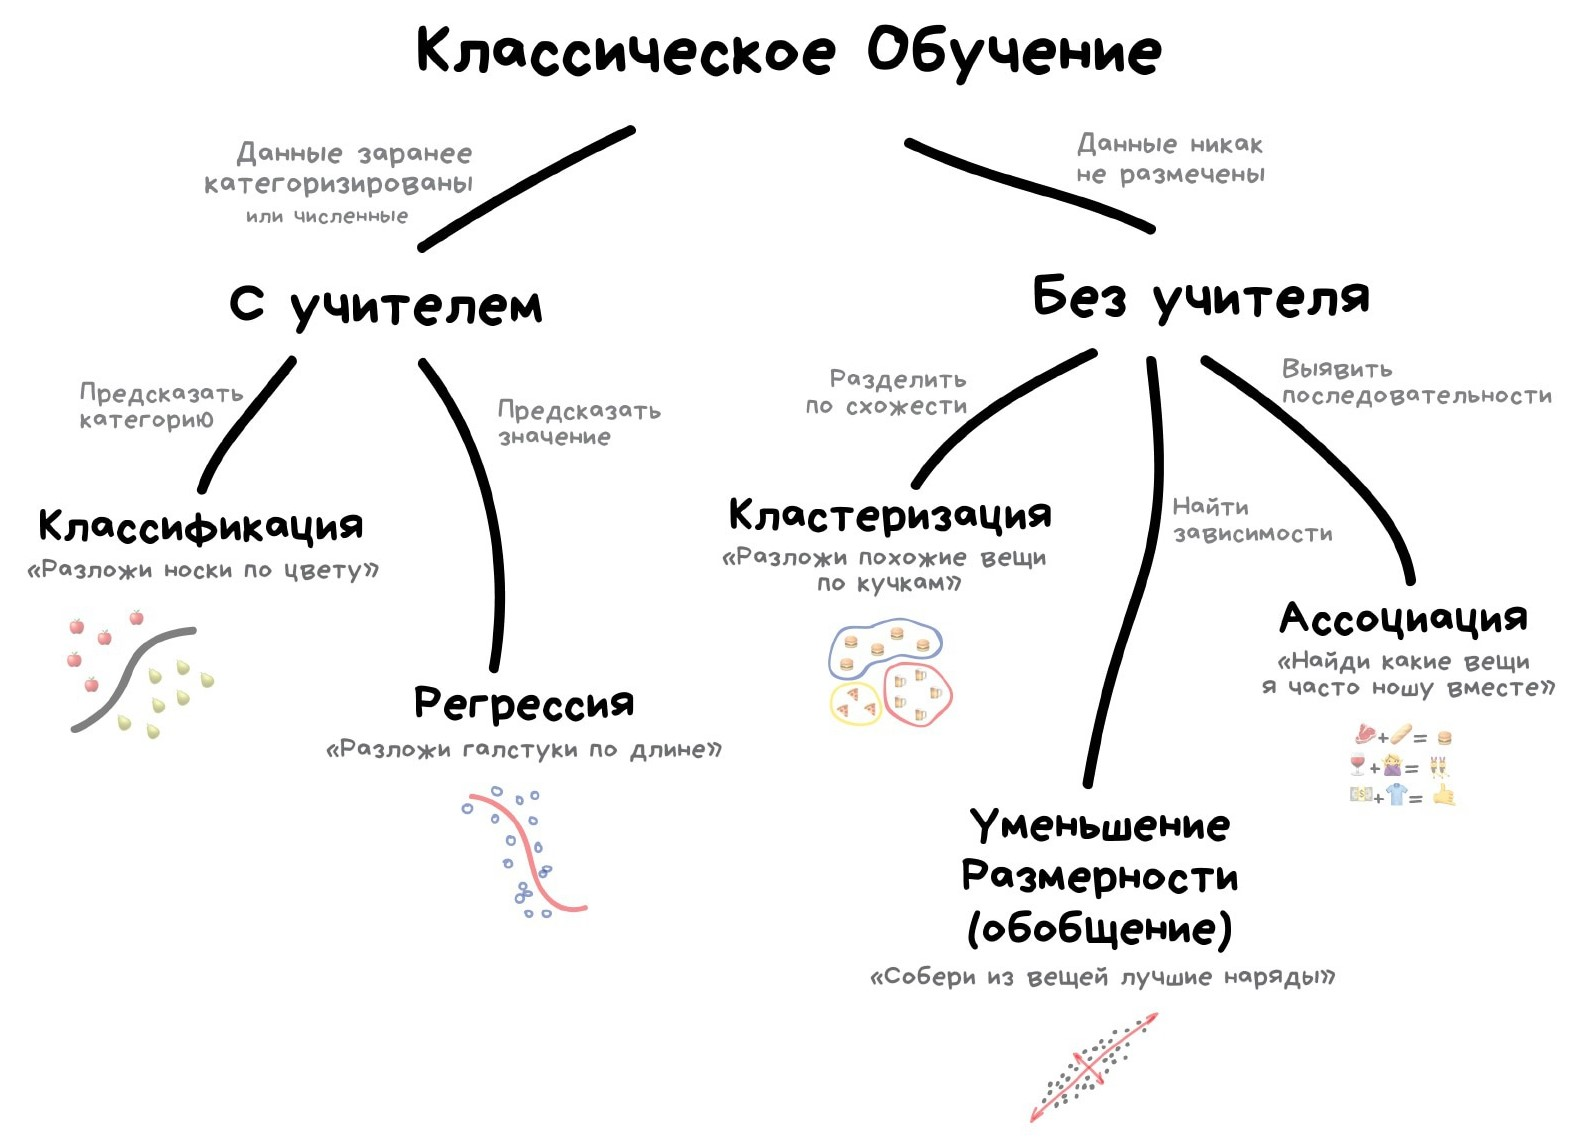
\includegraphics[width=.67\linewidth]{figures/fig5-supervised-learning.jpg}
\end{frame}

\begin{frame}{Другие задачи в терминах классификации и регрессии}
    \centering
    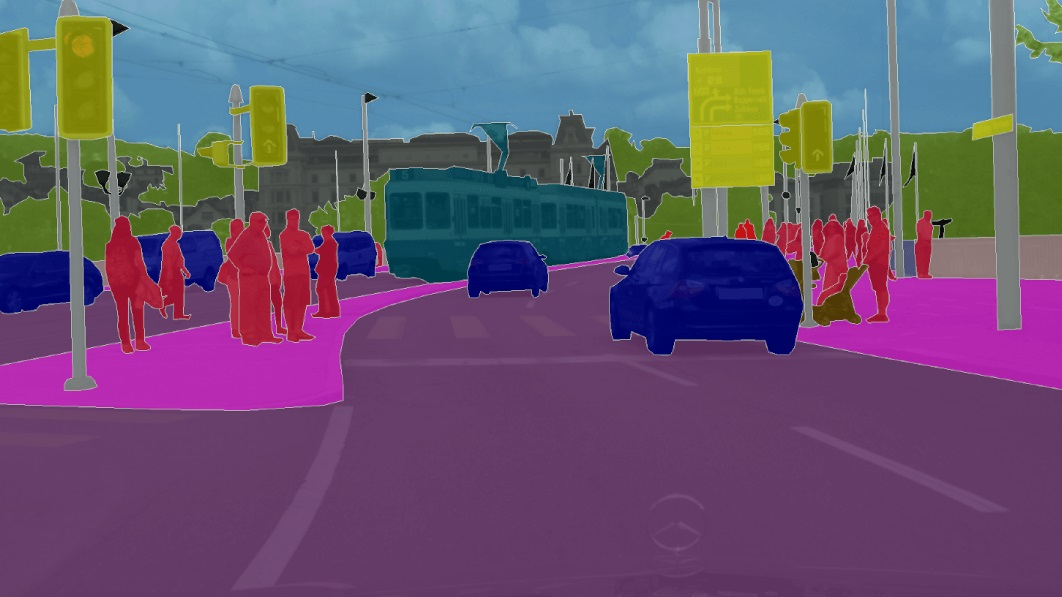
\includegraphics[width=.78\linewidth]{figures/fig6-segmentation.jpg} \\
    Задача семантической сегментации (semantic segmentation)
\end{frame}

\begin{frame}{Другие задачи в терминах классификации и регрессии}
    \centering
    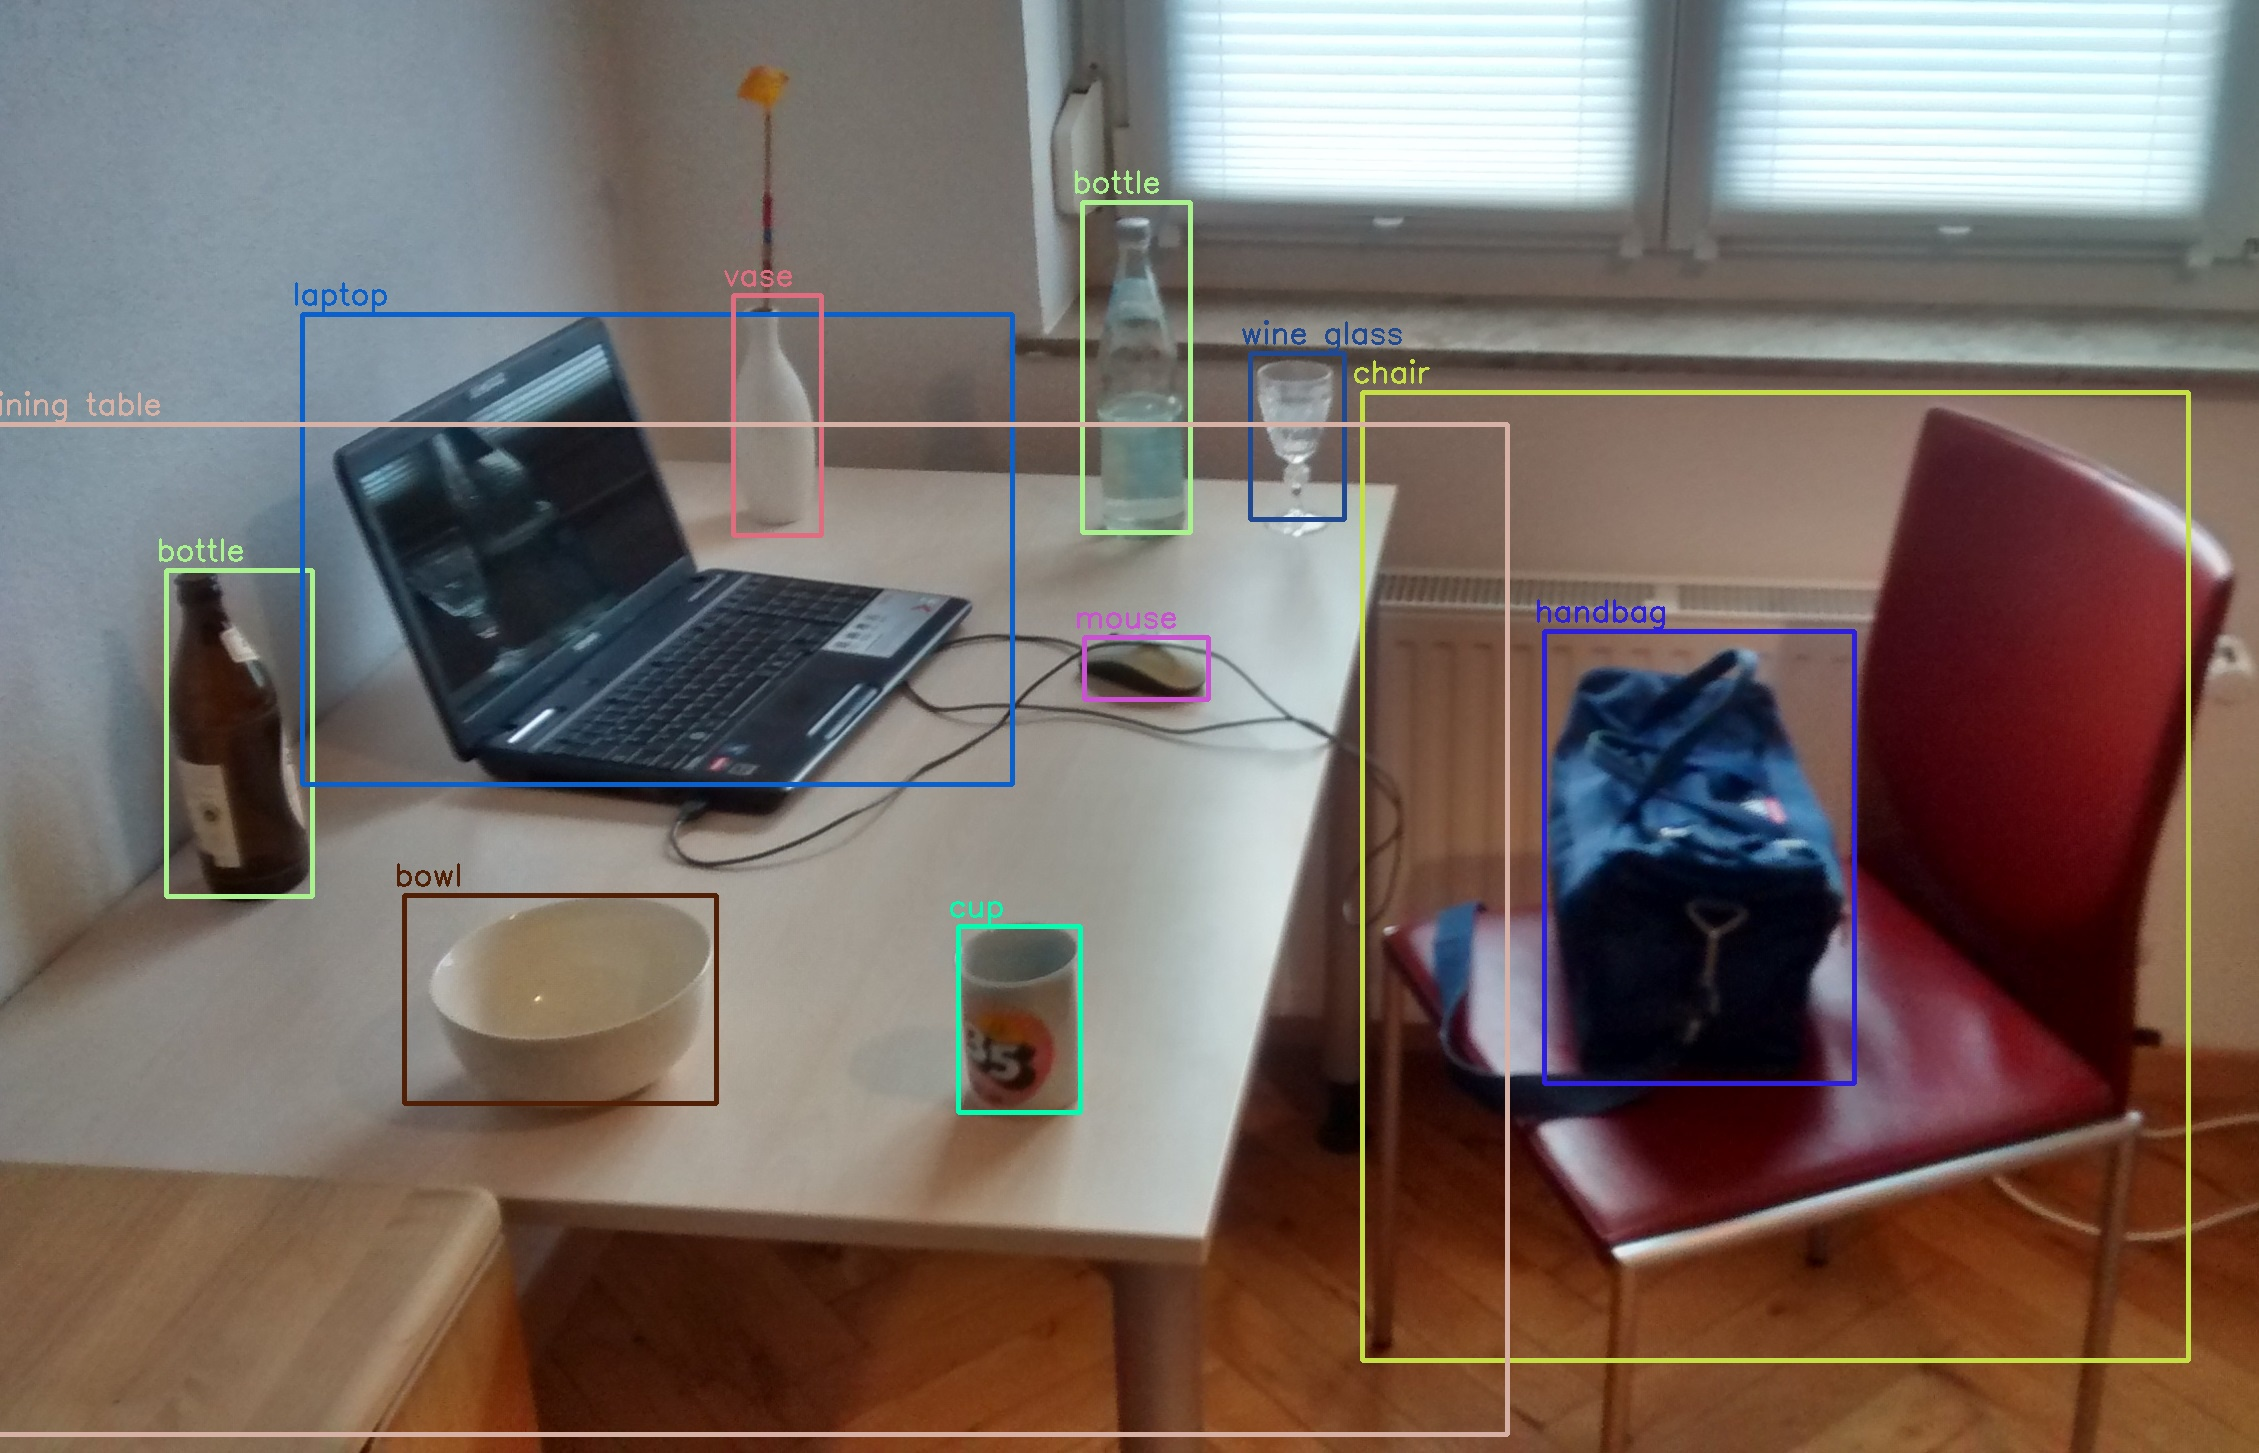
\includegraphics[width=.68\linewidth]{figures/fig7-object-detection.jpg} \\
    Задача детектирования объектов (object detection)
\end{frame}

\begin{frame}{Другие задачи в терминах классификации и регрессии}
    \centering
    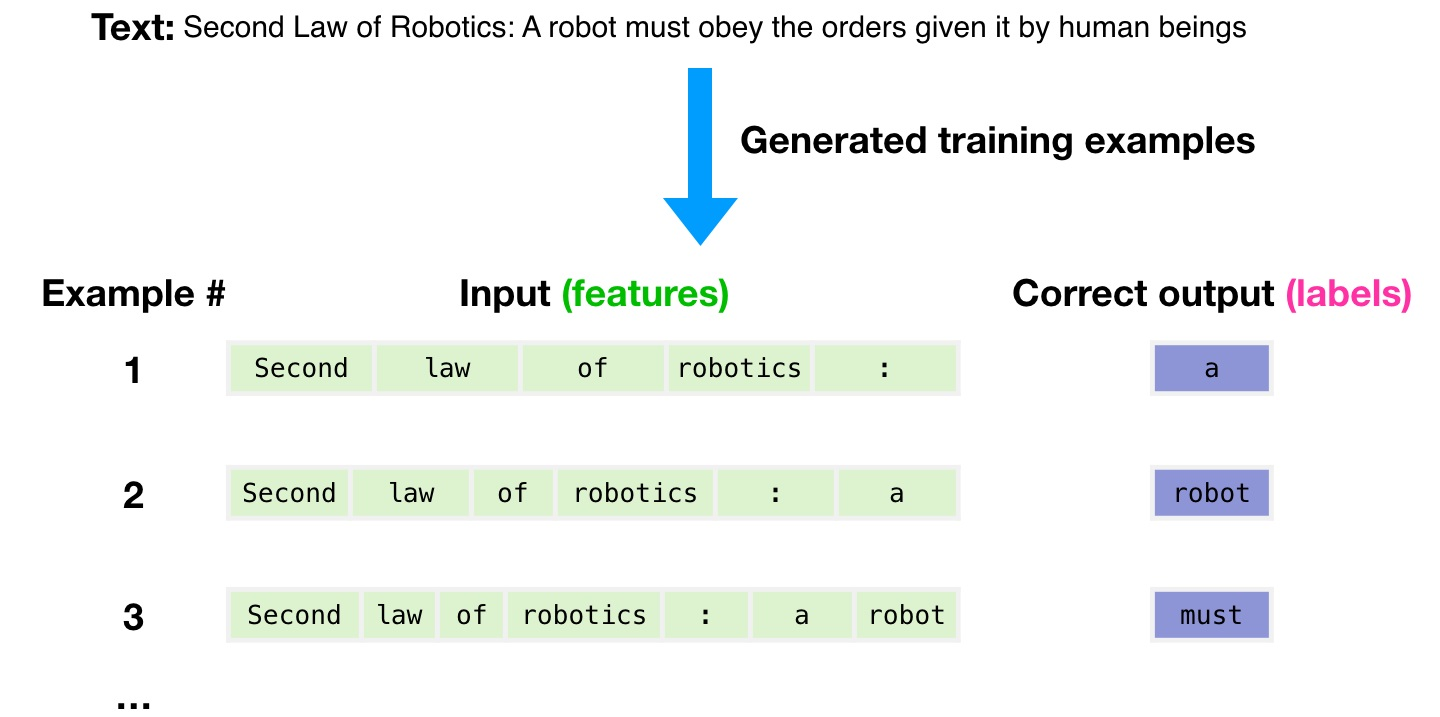
\includegraphics[width=.75\linewidth]{figures/fig8-lm.jpg} \\
    Задача языкового моделирования (language modeling)
\end{frame}

\begin{frame}{Python и производительность}
    Особенности языка Python:
    \begin{outline}
        \1 Интерпретируемый
        \1 Имеет динамическию сильную типизацию
        \1 Автоматически управленяет памятью (garbage collector)
        \1 Медленнее C++ в 10-10000 раз
        \1 Ограниченный параллелизм (GIL)
    \end{outline}
\end{frame}

\begin{frame}{Python и производительность}
    Python - язык-"клей": \\
    
\includegraphics[width=.9\linewidth]{figures/fig9-libraries.jpg}
\end{frame}
\end{document}